\chapter{Apéndices}
\label{chap:apendices}

\section{Apéndice 1: Guía de salas}
\label{anexo:guia-salas}

\drop{E}{  n} las páginas siguientes se adjunta la primera versión de la estructura de las salas del museo que fue propuesta al inicio del proyecto junto a su disposición y sus cuadros.

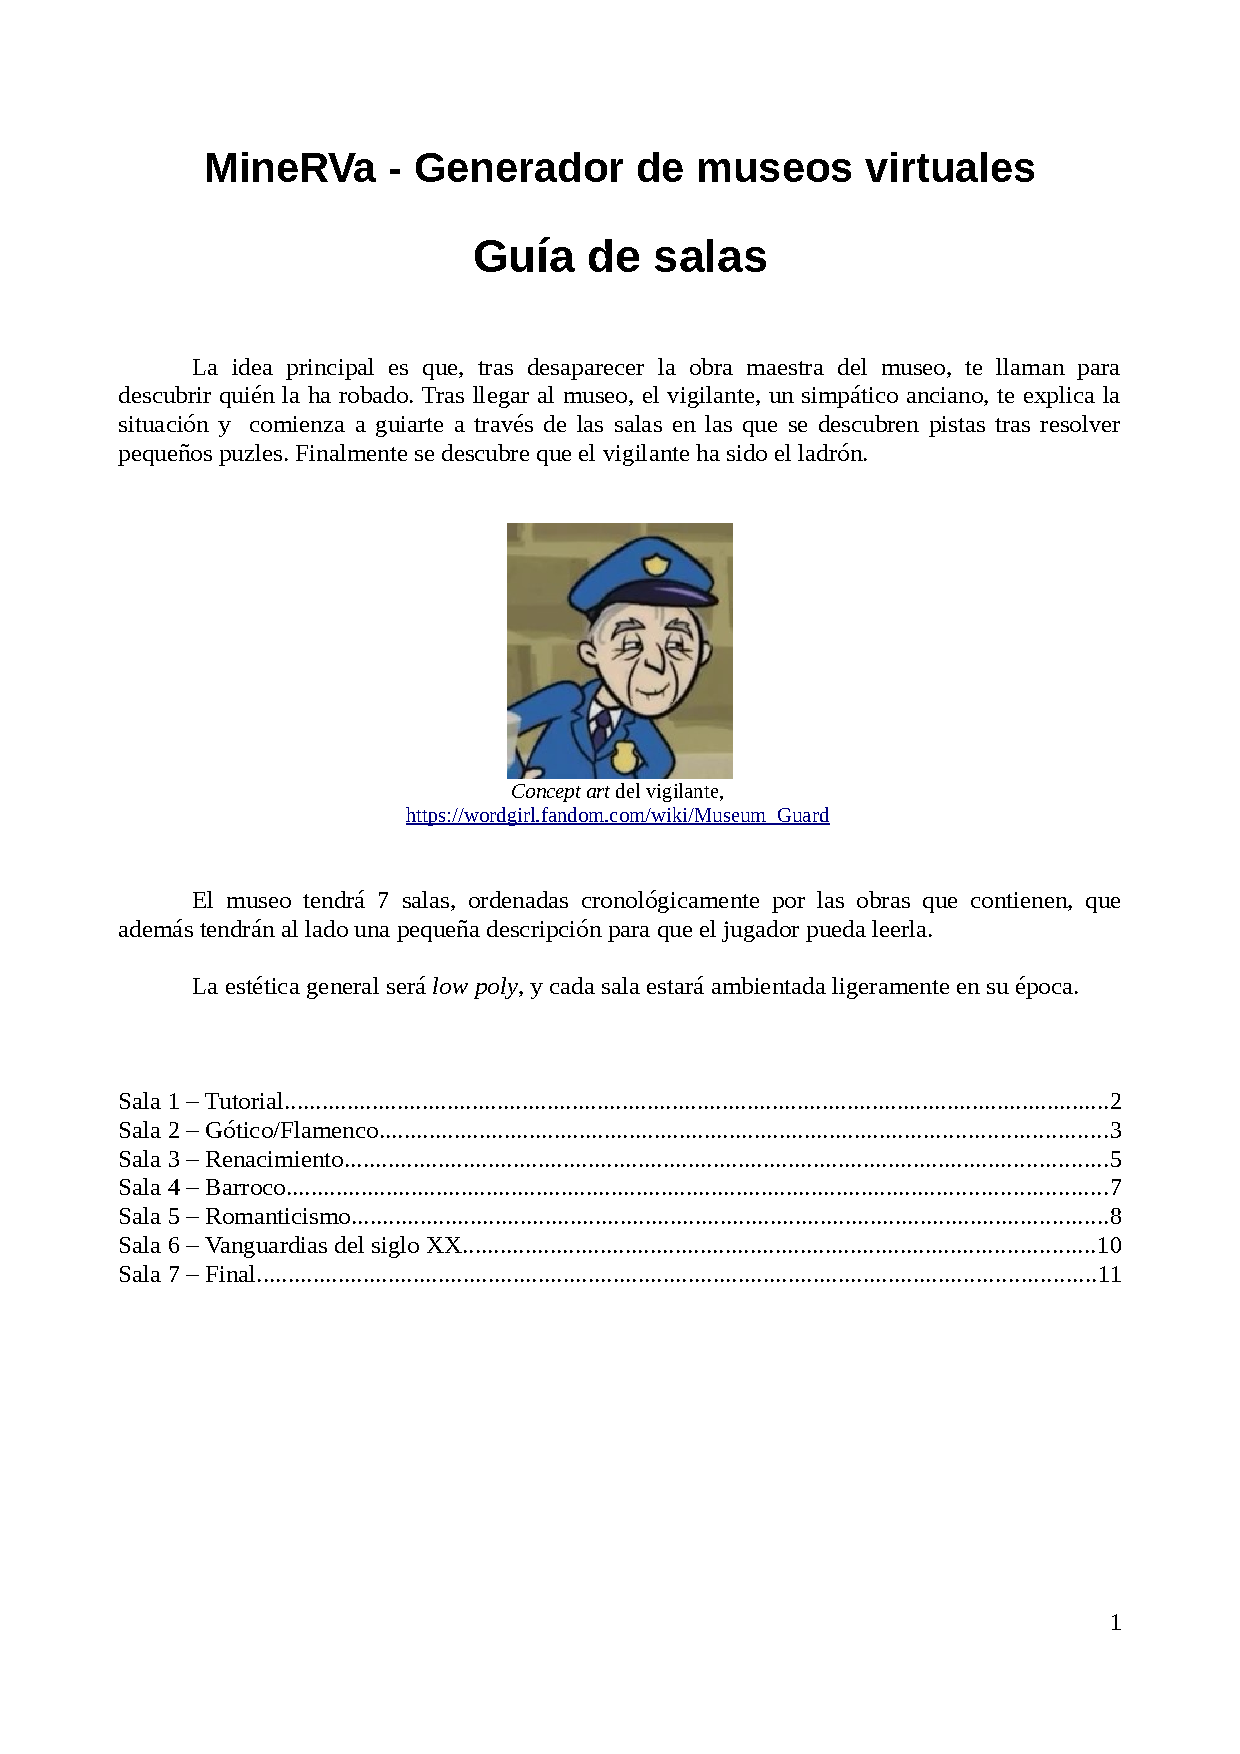
\includepdf[pages=-]{anexos/guia-salas.pdf}


\section{Apéndice 2: Game Design Document}
\label{anexo:gdd}

A continuación se adjunta el \acs{GDD} final de \textit{MineRVa}.

\newpage

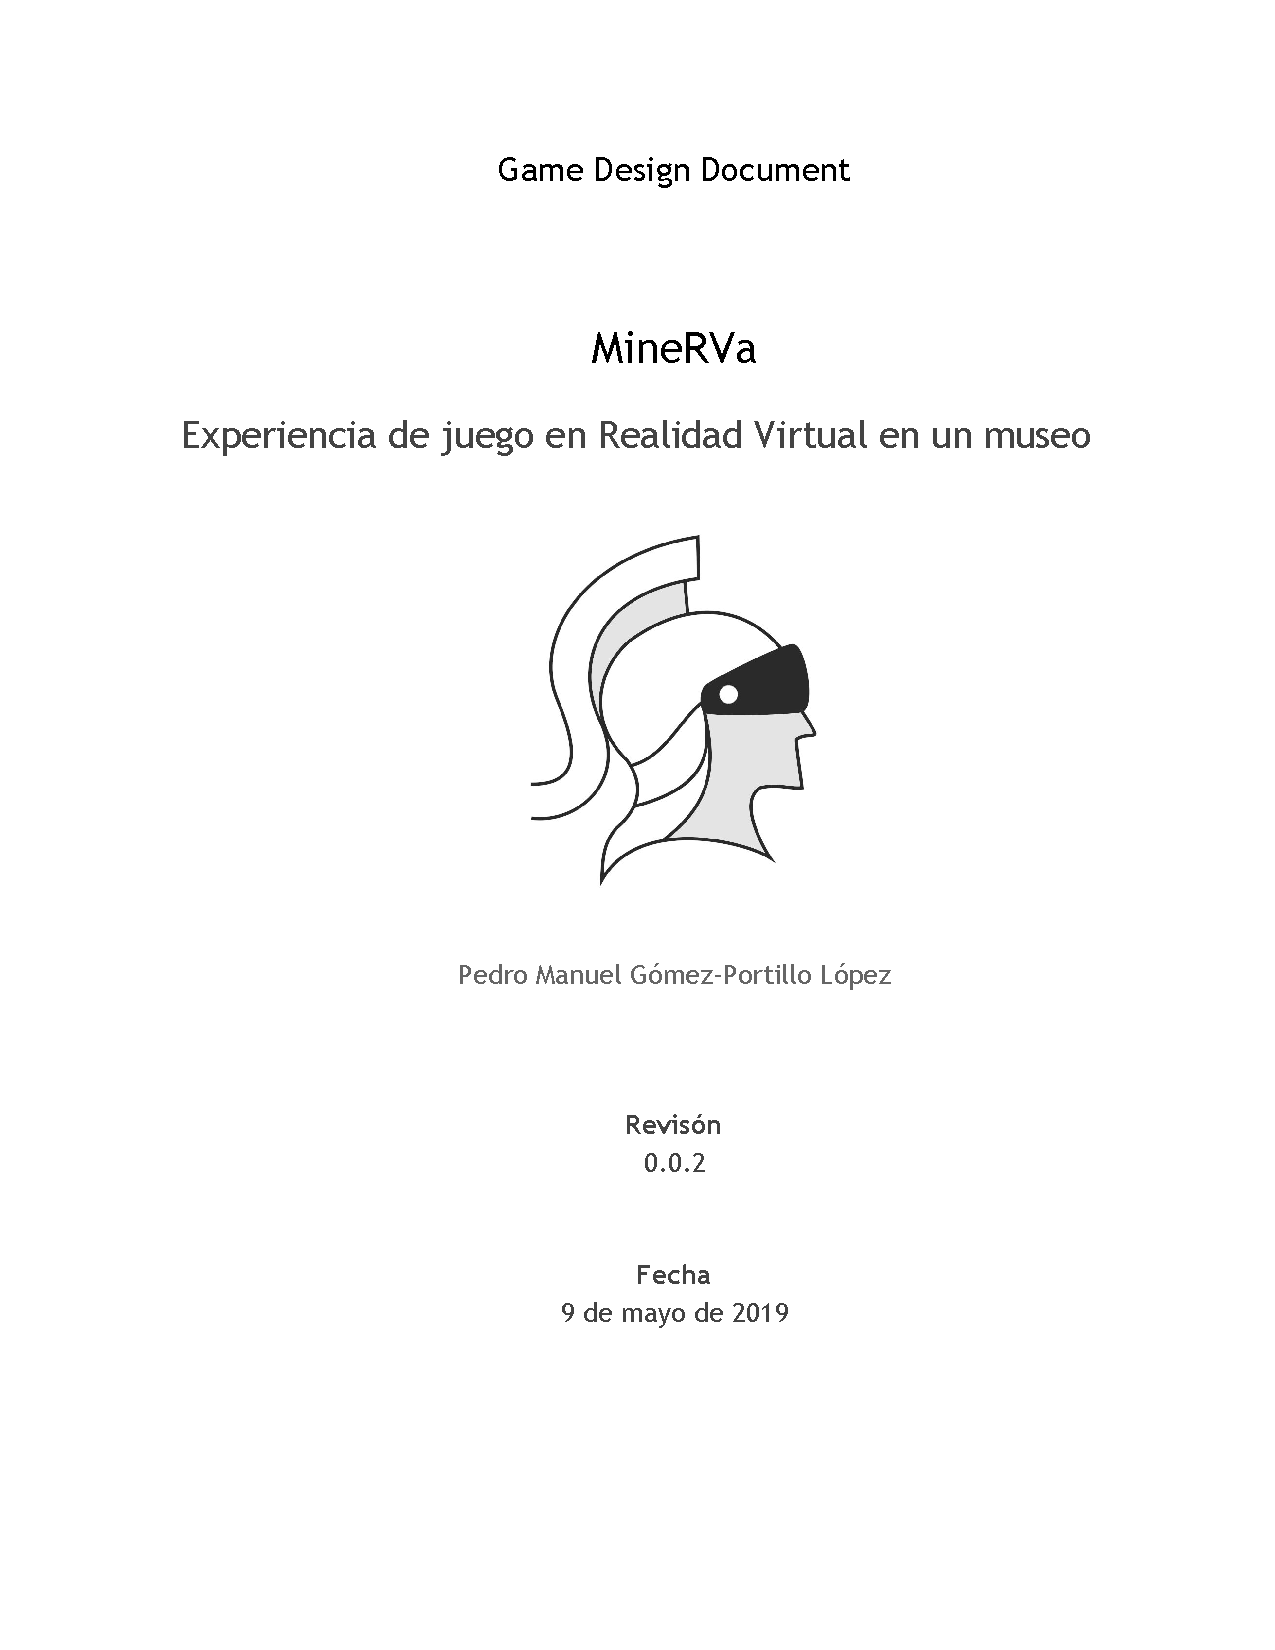
\includepdf[pages=-]{anexos/MineRVa-GDD.pdf}


\section{Apéndice 3: Evaluación de satisfacción con usuarios}
\label{anexo:evaluacion-satisfaccion}

A continuación se adjuntan los cuestionarios resueltos de las evaluaciones de satisfacción de los usuarios.

\newpage

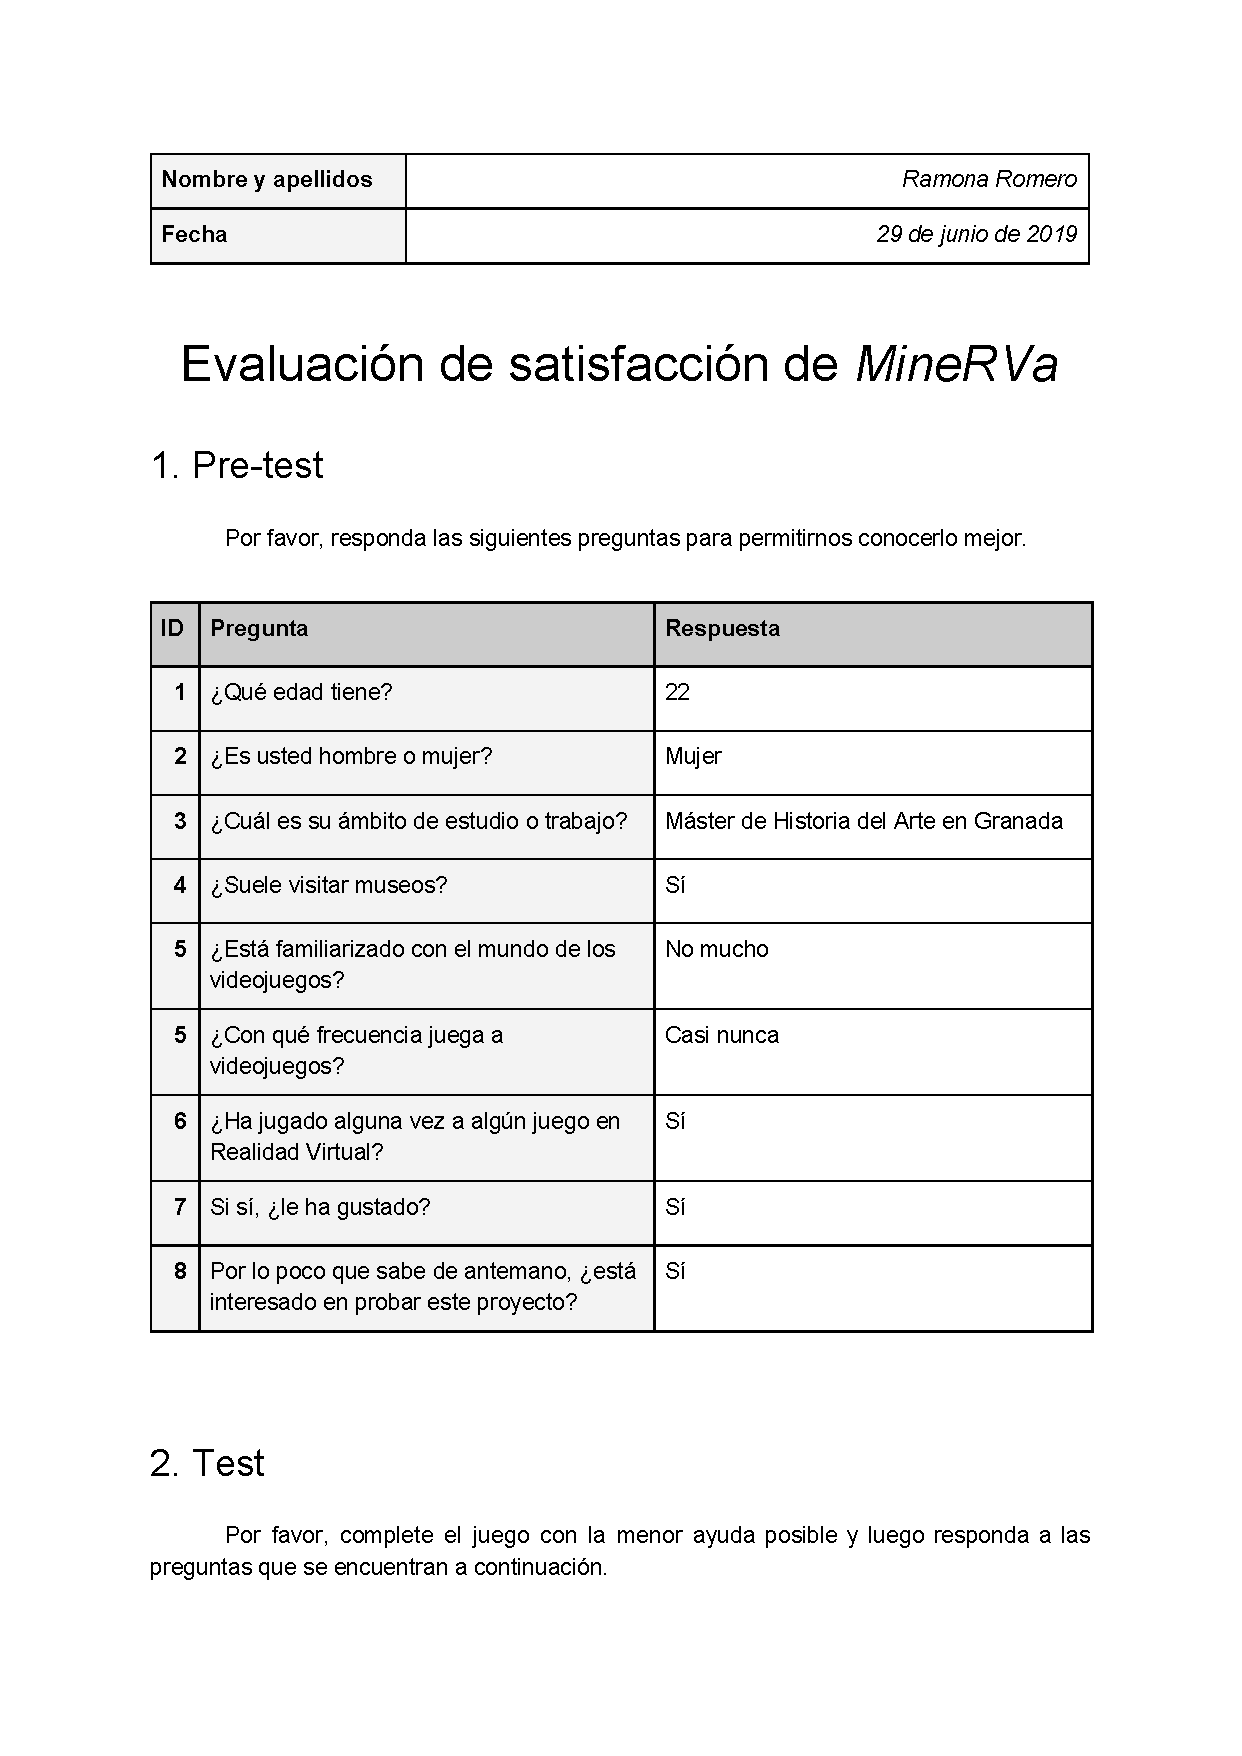
\includepdf[pages=-]{anexos/evaluacion_usuarios.pdf}

\newpage

\section{Agradecimientos}


Me gustaría dar por concluido este máster con unas pequeñas líneas en las que tener la oportunidad de recordar a todas las personas que han hecho posible de un modo u otro este \acs{TFM}.

Antes de nada, me gustaría agradecer al doctor Francisco Gutiérrez su orientación, motivación y tutela a lo largo del desarrollo de este proyecto.

También me gustaría recordar a todos los amigos que he conocido durante este año, tanto en clase como en las prácticas. Especialmente, a Juan Carlos Serrano y a Felipe Peiró; sin ellos, este curso no habría sido lo mismo.

Agradecer también a todos los amigos que han estado conmigo desde pequeño; a Álvaro, Jaime, Edu y a todos los demás. Y, por supuesto, a mi historiadora del arte personal.

Y por último, me gustaría dedicarles estas últimas líneas a mis padres, por todo lo que me han enseñado.

Gracias a todos.